\documentclass[mathserif,11pt]{beamer}

\mode<presentation>
{
\usetheme{default}
}


\title[] % (optional, use only with long paper titles)
{A Presentation on \LaTeX}


\author[Neil Armstrong]
{
  Neil Armstrong
}

\institute[]
{
  Jyothi Engineering College, Cheruthuruthy
}


% Includes for frame package
\usepackage{framed,color}
\definecolor{shadecolor}{rgb}{0.5,0.5,0.5}

% Make a custom block
\newenvironment<>{customBlock}[1]{%
  \begin{actionenv}#2%
      \def\insertblocktitle{#1}%
      \par%
      \mode<presentation>{%
        \setbeamercolor{block title}{fg=white,bg=orange!20!black}
       \setbeamercolor{block body}{fg=black,bg=olive!50}
       \setbeamercolor{itemize item}{fg=orange!20!black}
       \setbeamertemplate{itemize item}[triangle]
     }%
      \usebeamertemplate{block begin}}
    {\par\usebeamertemplate{block end}\end{actionenv}}


% Define new environments for mdframed package
\usepackage{tikz}
\usepackage[framemethod=tikz]{mdframed}
\usepackage{multirow}
\usepackage{graphicx}

\newmdenv[tikzsetting={draw=black,fill=white,fill opacity=0.7, line width=0.5pt},backgroundcolor=none,leftmargin=0,rightmargin=0,innertopmargin=4pt,skipbelow=\baselineskip,%
skipabove=\baselineskip]{TitleBox}

%----------------------------------------------------------------------------------------
\begin{document}
%------------------------------------------------------------------------
% Title Frame - Do not edit
{ \usebackgroundtemplate{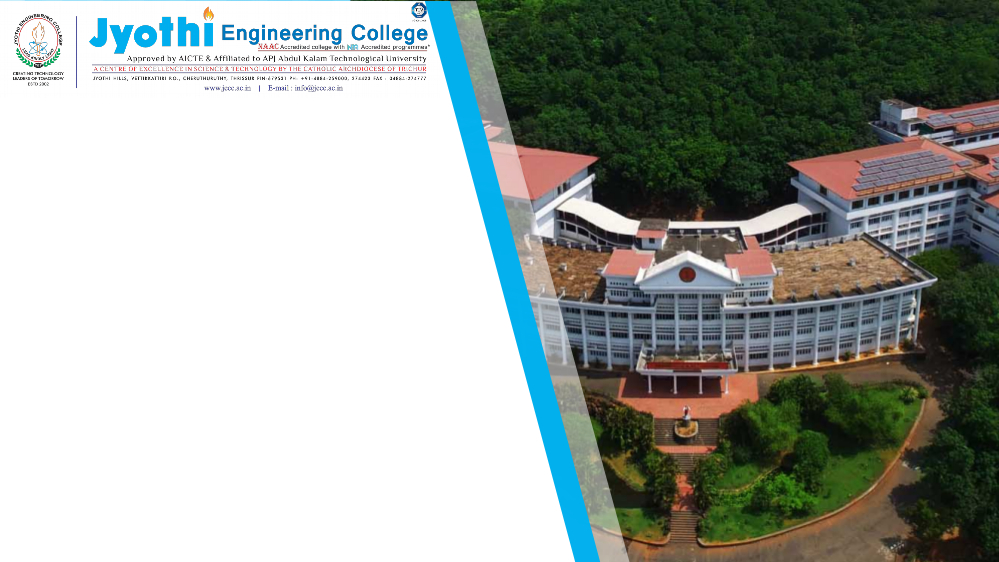
\includegraphics[width=1.0\paperwidth]{backgroundimages/one.jpg}}
  \begin{frame}[plain] 
  \begin{TitleBox}
  \maketitle  
  \end{TitleBox}
  \end{frame}
}
%------------------------------------------------------------------------
%Contents Frame - Edit contents
\usebackgroundtemplate{
\includegraphics[width=1.0\paperwidth]{backgroundimages/two.jpg}}
\begin{frame}
  \begin{TitleBox}
  \begin{itemize}
      \item first line
      \item second line
      \item third line
  \end{itemize}
  \end{TitleBox}
\end{frame}
%-----------------------------------------------------------------------
%Block Frame
{
  \usebackgroundtemplate{
\includegraphics[width=1.0\paperwidth]{backgroundimages/two.jpg}}
  \begin{frame}[plain] 

  \begin{tabular}{ |l|l|l| }
  \hline
  \multicolumn{3}{ |c| }{Team sheet} \\
  \hline
  Goalkeeper & GK & Paul Robinson \\ \hline
  \multirow{4}{*}{Defenders} & LB & Lucas Radebe \\
   & DC & Michael Duburry \\
   & DC & Dominic Matteo \\
   & RB & Didier Domi \\ \hline
  \multirow{3}{*}{Midfielders} & MC & David Batty \\
   & MC & Eirik Bakke \\
   & MC & Jody Morris \\ \hline
  Forward & FW & Jamie McMaster \\ \hline
  \multirow{2}{*}{Strikers} & ST & Alan Smith \\
   & ST & Mark Viduka \\
  \hline
  \end{tabular}


  \end{frame}
}

%---------------------------------------------
%Block Frame
{
  \usebackgroundtemplate{
\includegraphics[width=1.0\paperwidth]{backgroundimages/three.jpg}}
  \begin{frame}[plain] 

  \begin{TitleBox}
  This is a sample block to test the contents against a background.
  \end{TitleBox}

  \end{frame}
}
%----------------------------------------------------------------
  %Block Frame
{
  \usebackgroundtemplate{
\includegraphics[width=1.0\paperwidth]{backgroundimages/three.jpg}}
  \begin{frame}[plain] 
  \begin{center}
  
\includegraphics[width=5cm]{presentationimages/bullet.jpg}
  \end{center}
  \end{frame}
}
%----------------------------------------------------------------
%----------------------------------------------------------------

%Another Frame
{
  \usebackgroundtemplate{
\includegraphics[width=1.0\paperwidth]{backgroundimages/three.jpg}}
  \begin{frame}[plain] 

  \begin{customBlock}{A customized  block}
    Using block option
  \end{customBlock}

  \end{frame}
}
%----------------------------------------------------------------

% Last Frame
{
 \usebackgroundtemplate{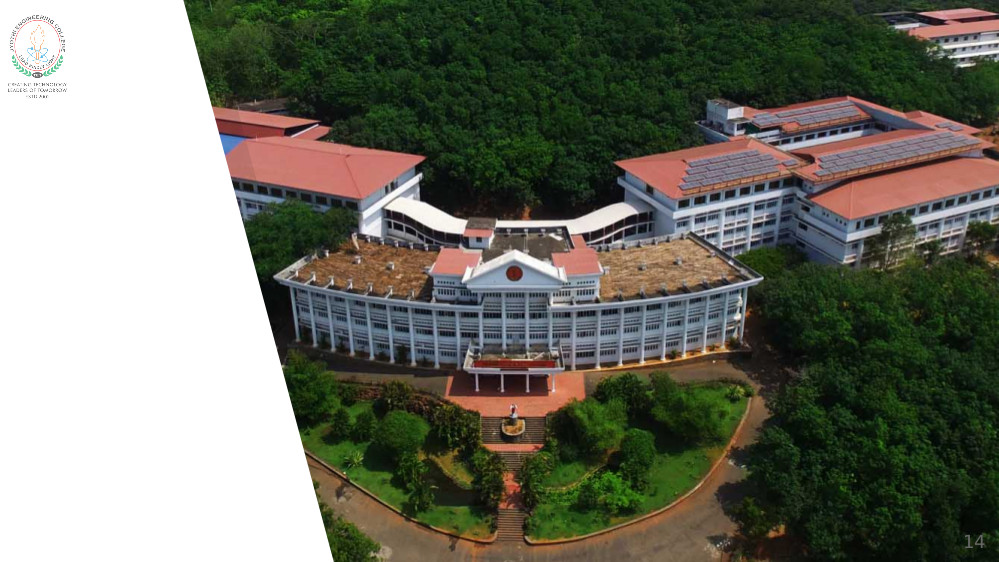
\includegraphics[width=1.0\paperwidth]{backgroundimages/six.jpg}}
  \begin{frame}[plain] 

  \begin{TitleBox}
   \begin{center}
   Thank you  
   \end{center}
  \end{TitleBox}

  \end{frame}
}


%-----------------------------------
\end{document}